\documentclass{beamer}
\usetheme{Madrid}
\usecolortheme{default}

% Required packages
\usepackage{graphicx}
\usepackage{hyperref}
\usepackage{tikz}        % <-- ADDED: Required for tikzpicture environment
\usetikzlibrary{shapes, arrows, positioning} % <-- ADDED: For better flowchart styling

% Title Page Information
\title{Effective Wiki Search Strategy}
\subtitle{Finding the Right Information for Your Task}
\author{Your Team Name}
\date{September 2026}

\begin{document}
	
	% --- Slide 1: Title ---
	\begin{frame}
		\titlepage
	\end{frame}
	
	% --- Slide 2: Table of Contents ---
	\begin{frame}{Agenda}
		\tableofcontents
	\end{frame}
	
	% --- Slide 3: Introduction & The Problem ---
	\section{Introduction}
	\begin{frame}{The Challenge: Finding the Right Page}
		\begin{block}{The Core Problem}
			How do we efficiently search for specific procedures (e.g., \texttt{pip setup}) on the Wiki?
		\end{block}
		\begin{itemize}
			\item Many teams contribute to the Wiki.
			\item Information evolves over time.
			\item The \textbf{best} page is not always the \textbf{newest} page.
			\item We need to balance historical context (our team's past work) with recent updates (other teams).
		\end{itemize}
		\begin{alertblock}{Example Task}
			Setting up \texttt{pip} for bootstrapping and package installation.
		\end{alertblock}
	\end{frame}
	
	% --- Slide 4: The Dual Approach ---
	\section{The Dual Strategy}
	\begin{frame}{The Search Strategy: A Dual Approach}
		\begin{figure}
			\centering
			% Simple visual representation using text blocks
			\begin{minipage}{0.45\textwidth}
				\begin{block}{1. Our Team's History}
					\centering
					\textbf{Historical Context}\\
					\vspace{0.5cm}
					\textcolor{blue}{Know Our Pages}\\
					\textcolor{blue}{Review Past Solutions}
				\end{block}
			\end{minipage}
			\hfill
			\begin{minipage}{0.45\textwidth}
				\begin{block}{2. Other Teams' Updates}
					\centering
					\textbf{Current Innovations}\\
					\vspace{0.5cm}
					\textcolor{orange}{Find Recent Edits}\\
					\textcolor{orange}{Adapt to Changes}
				\end{block}
			\end{minipage}
		\end{figure}
		\vspace{1cm}
		\begin{center}
			\textsc{Goal: Synthesize both to select the best page and update it.}
		\end{center}
	\end{frame}
	
	% --- Slide 5: Step 1 - Know Your Team ---
	\section{Step 1: Know Your Territory}
	\begin{frame}{Step 1: Understanding "Our" Pages}
		\begin{enumerate}
			\item \textbf{Identify Servers/Projects:} Know which servers or projects belong to your team.
			\item \textbf{Filter by Ownership:} Use Wiki filters to show pages authored or primarily used by your team.
			\item \textbf{Find the "Last Time":} Locate the page your team used the last time this task was performed (e.g., last \texttt{pip} setup).
		\end{enumerate}
		\begin{exampleblock}{Why this matters}
			This ensures you understand the \textit{baseline} and \textit{terminology} your team is familiar with before looking at external changes.
		\end{exampleblock}
	\end{frame}
	
	% --- Slide 6: Step 2 - Explore the Wider Wiki ---
	\section{Step 2: Explore the Universe}
	\begin{frame}{Step 2: Searching the "Universal" Wiki}
		\begin{itemize}
			\item \textbf{Broad Search:} Search for the specific task (e.g., "pip setup", "bootstrap packages").
			\item \textbf{Identify Creators:} Check \textit{which team} created the page. Newer pages are often created by other teams working on modern architecture.
			\item \textbf{Review Timestamps:} Look for pages updated recently (e.g., within the last 2-6 months).
		\end{itemize}
		\begin{block}{Key Insight}
			"Other teams have the latest pages." They might have solved a new dependency issue or changed a registry URL that we need to adopt.
		\end{block}
	\end{frame}
	
	% --- Slide 7: Step 3 - Comparative Analysis ---
	\section{Step 3: Synthesize Information}
	\begin{frame}{Step 3: Comparing and Selecting the Best Page}
		\begin{table}
			\centering
			\begin{tabular}{|l|c|c|}
				\hline
				\textbf{Criteria} & \textbf{Our Old Page} & \textbf{Other Team's New Page} \\
				\hline
				Date Updated & 2024 & 2026 \\
				\hline
				Pip Version & 20.x & 24.x \\
				\hline
				Bootstrap Method & Manual & Automated Script \\
				\hline
				Known Issues & Outdated & Resolved \\
				\hline
			\end{tabular}
			\caption{Comparison Matrix}
		\end{table}
		\vspace{0.5cm}
		\begin{enumerate}
			\item Identify the \textbf{core workflow} that remains the same.
			\item Note the \textbf{new improvements} (e.g., new flags, new repositories).
			\item Select the page that is \textbf{most accurate} for the current environment.
		\end{enumerate}
	\end{frame}
	
	% --- Slide 8: Decision Flowchart ---
	\section{Decision Logic}
	\begin{frame}{Decision Flowchart for Wiki Search}
		\begin{center}
			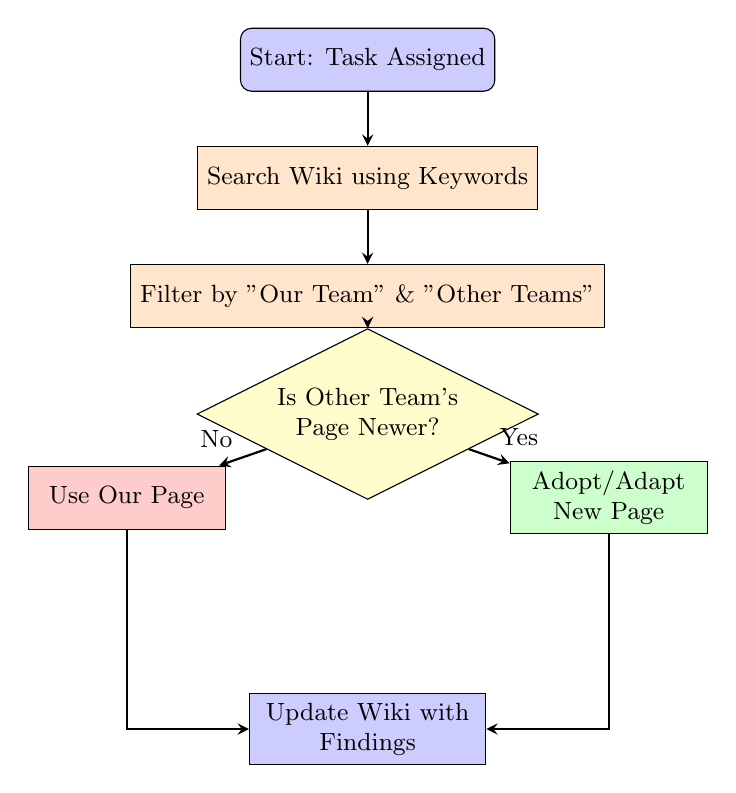
\begin{tikzpicture}[
				node distance=1.5cm and 2cm,
				every node/.style={font=\small},
				startstop/.style={rectangle, rounded corners, draw, fill=blue!20, minimum width=3cm, minimum height=0.8cm, align=center},
				process/.style={rectangle, draw, fill=orange!20, minimum width=3cm, minimum height=0.8cm, align=center},
				decision/.style={diamond, draw, fill=yellow!20, minimum width=3cm, minimum height=0.8cm, align=center, aspect=2},
				ourpage/.style={rectangle, draw, fill=red!20, minimum width=2.5cm, minimum height=0.8cm, align=center},
				newpage/.style={rectangle, draw, fill=green!20, minimum width=2.5cm, minimum height=0.8cm, align=center},
				final/.style={rectangle, draw, fill=blue!20, minimum width=3cm, minimum height=0.8cm, align=center},
				arrow/.style={thick, ->, >=stealth}
				]
				% Nodes
				\node (start) [startstop] {Start: Task Assigned};
				\node (step1) [process, below of=start] {Search Wiki using Keywords};
				\node (step2) [process, below of=step1] {Filter by "Our Team" \& "Other Teams"};
				\node (step3) [decision, below of=step2] {Is Other Team's\\Page Newer?};
				\node (step4a) [ourpage, below left of=step3, xshift=-2cm] {Use Our Page};
				\node (step4b) [newpage, below right of=step3, xshift=2cm] {Adopt/Adapt\\New Page};
				\node (step5) [final, below of=step3, yshift=-2.5cm] {Update Wiki with\\Findings};
				
				% Arrows
				\draw [arrow] (start) -- (step1);
				\draw [arrow] (step1) -- (step2);
				\draw [arrow] (step2) -- (step3);
				\draw [arrow] (step3) -- node[above left] {No} (step4a);
				\draw [arrow] (step3) -- node[above right] {Yes} (step4b);
				\draw [arrow] (step4a) |- (step5);
				\draw [arrow] (step4b) |- (step5);
			\end{tikzpicture}
		\end{center}
	\end{frame}
	
	% --- Slide 9: The End Goal ---
	\section{Conclusion}
	\begin{frame}{The Final Outcome: Updating the Wiki}
		\begin{block}{The End Goal}
			\begin{center}
				\Large
				\textbf{Select the best page and put it on the wiki page.}
			\end{center}
		\end{block}
		\begin{itemize}
			\item Consolidate the old workflow with the new changes.
			\item Ensure the page is \textbf{reusable} for future searches.
			\item Create a standard "How-To" for future team members.
		\end{itemize}
		\begin{alertblock}{Remember}
			The search is not just about finding \textit{any} page. It is about finding the \textit{right} page that represents the collective knowledge of the organization.
		\end{alertblock}
	\end{frame}
	
	% --- Slide 10: Summary & Q&A ---
	\section{Q\&A}
	\begin{frame}{Summary \& Questions}
		\begin{columns}[T]
			\begin{column}{.5\textwidth}
				\textbf{Key Takeaways}
				\begin{enumerate}
					\item Know your team's servers and pages.
					\item Look at other teams' recent updates.
					\item Compare the workflow and identify changes.
					\item Select and refresh the best page.
				\end{enumerate}
			\end{column}
			\begin{column}{.5\textwidth}
				\begin{center}
					\includegraphics[width=0.8\textwidth]{example-image} % Placeholder for a diagram
					
					\textit{Search. Compare. Update.}
				\end{center}
			\end{column}
		\end{columns}
		\vspace{1cm}
		\begin{center}
			\Huge \textcolor{blue}{?} \\
			\Large Thank You
		\end{center}
	\end{frame}
	
\end{document}